\chapter{Motor Learning and Adaptation}
\label{ch:motor-learning}

\epigraph{%
  Practice does not make perfect.
  Practice makes permanent.
  Only perfect practice makes perfect.
}{}

\section{Three Learning Systems}

Motor learning involves three distinct neural systems with different timescales and mechanisms:

\begin{enumerate}
  \item \textbf{Error-based learning} (cerebellum): uses sensory prediction errors (climbing
        fiber signals) to update cerebellar forward models via LTD (Marr, 1969; Kawato et al.,
        1987). Trial-by-trial timescale (minutes to hours). Dominant mechanism for visuomotor
        adaptation (Shadmehr and Mussa-Ivaldi, 1994).

  \item \textbf{Reinforcement learning} (basal ganglia): uses dopamine reward signals to
        strengthen successful motor patterns (Schultz et al., 1997). Slower than error-based
        learning (hours to days). Enables discovery of novel solutions not implicit in the
        task structure.

  \item \textbf{Consolidation and structural learning} (cortical): repetition of a movement
        biases future movements toward repeated patterns (Cohen et al., 2005). Timescale of
        hours to days; explains habit formation. Involves gradual changes in M1 tuning and
        synaptic weights.
\end{enumerate}

\begin{figure}[h]
\centering
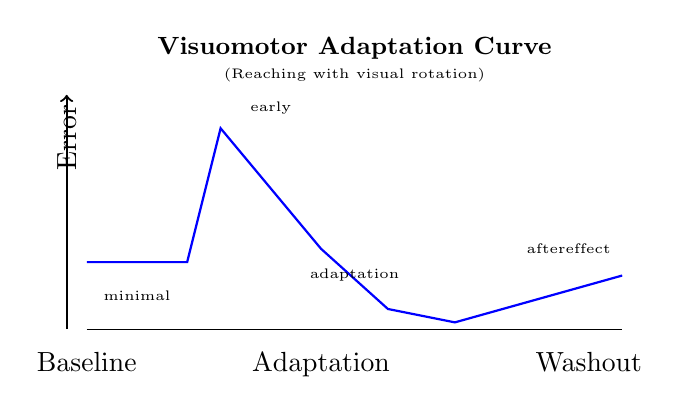
\begin{tikzpicture}[scale=0.85]
  % Timeline
  \draw (0, 0) -- (8, 0);
  \draw (0, -0.2) node[align=center, anchor=north] {Baseline};
  \draw (3.5, -0.2) node[align=center, anchor=north] {Adaptation};
  \draw (7.5, -0.2) node[align=center, anchor=north] {Washout};

  % Error curve (schematic)
  \draw[blue, thick] (0, 1) -- (1.5, 1) -- (2, 3) -- (3.5, 1.2) -- (4.5, 0.3) -- (5.5, 0.1) -- (8, 0.8);

  % Labels
  \draw (0.75, 0.5) node[align=center, anchor=center, font=\tiny] {minimal};
  \draw (2.75, 3.3) node[align=center, anchor=center, font=\tiny] {early};
  \draw (4, 0.8) node[align=center, anchor=center, font=\tiny] {adaptation};
  \draw (7.2, 1.2) node[align=center, anchor=center, font=\tiny] {aftereffect};

  % Dashed line (zero)
  \draw[dashed] (0, 0) -- (8, 0);

  % Y-axis
  \draw[->, thick] (-0.3, 0) -- (-0.3, 3.5) node[align=center, anchor=east, rotate=90] {Error};

  % Title
  \draw (4, 4.2) node[align=center, anchor=center, font=\small\bf] {Visuomotor Adaptation Curve};
  \draw (4, 3.8) node[align=center, anchor=center, font=\tiny] {(Reaching with visual rotation)};
\end{tikzpicture}
\caption{Characteristic visuomotor adaptation profile (Shadmehr and Mussa-Ivaldi, 1994):
rapid error reduction (first 20 trials), gradual asymptote, persistent aftereffect
demonstrating learning consolidation.}
\label{fig:ch9:visuomotor-adaptation}
\end{figure}

\section{Visuomotor Adaptation}

The classic paradigm for studying error-based learning (Kamin, 1969; Shadmehr and Mussa-Ivaldi,
1994):

\begin{lstlisting}[language=Python, caption={Visuomotor adaptation simulation.}]
import numpy as np

def simulate_visuomotor_adaptation(
    n_baseline: int = 50,
    n_adaptation: int = 200,
    n_washout: int = 100,
    perturbation_deg: float = 30.0,
    learning_rate: float = 0.05,
    retention: float = 0.98
) -> dict:
    """Simulate visuomotor rotation adaptation.

    A simple state-space model of adaptation:
    x_{k+1} = retention * x_k + learning_rate * e_k

    Parameters
    ----------
    n_baseline : int
        Baseline trials (no perturbation).
    n_adaptation : int
        Adaptation trials (perturbation on).
    n_washout : int
        Post-adaptation trials (perturbation off).
    perturbation_deg : float
        Rotation perturbation in degrees.
    learning_rate : float
        Rate of error-based learning.
    retention : float
        Memory retention between trials.

    Returns
    -------
    dict
        Keys: 'trial', 'reaching_error', 'internal_state',
              'phase' (labels for each trial)
    """
    n_total = n_baseline + n_adaptation + n_washout
    p = np.radians(perturbation_deg)

    # Internal state (learned compensation)
    x = 0.0
    errors = np.zeros(n_total)
    states = np.zeros(n_total)
    phases = []

    for trial in range(n_total):
        if trial < n_baseline:
            perturbation = 0.0
            phases.append('baseline')
        elif trial < n_baseline + n_adaptation:
            perturbation = p
            phases.append('adaptation')
        else:
            perturbation = 0.0
            phases.append('washout')

        # Reaching error = perturbation - compensation
        error = perturbation - x
        errors[trial] = np.degrees(error)
        states[trial] = np.degrees(x)

        # Update internal state
        x = retention * x + learning_rate * error

    return {
        'trial': np.arange(n_total),
        'reaching_error': errors,
        'internal_state': states,
        'phase': phases
    }


result = simulate_visuomotor_adaptation()
print("Visuomotor Adaptation Summary:")
print(f"  Baseline error:  {np.mean(np.abs(result['reaching_error'][:50])):.1f} deg")
print(f"  Final adaptation error: "
      f"{np.abs(result['reaching_error'][249]):.1f} deg")
print(f"  Aftereffect: {result['reaching_error'][250]:.1f} deg")
\end{lstlisting}

\section{Savings and Interference}

\subsection{Savings}
Re-learning a previously learned adaptation is faster than initial learning,
even after complete washout (Ebbinghaus, 1885; Huang et al., 2011). This savings
effect suggests that motor memories are not erased but suppressed, with additional
learning circuits retaining implicit information about the learning dynamics.

\subsection{Interference and Dual-Rate Learning}
Learning opposite perturbations (A then B) produces anterograde interference:
learning B slows retention of A (Li and Xie, 2000). This is explained by dual-rate
learning models: a fast process learns trial-by-trial; a slow process consolidates.
Interference occurs because the fast process is task-specific while the slow process
is more general.

\section{Structural Learning and Meta-Learning}

Over many adaptation experiences, subjects develop the ability to adapt faster---they
learn to learn (context-dependent learning). Smith et al. (1998) showed that prior
exposure to one visuomotor rotation task accelerates learning of a novel rotation.
This involves learning the structure of the task space itself, not just individual
parameter values. Brain areas like dorsolateral prefrontal cortex appear to encode
such meta-learning (Gershman et al., 2017).

\section*{Exercises}

\begin{enumerate}
  \item \textbf{State-Space Model.} Using the provided code, explore how learning
        rate and retention affect adaptation speed and aftereffect size.

  \item \textbf{Dual-Rate Model.} Implement a dual-rate model (fast + slow process)
        and show that it can explain savings.

  \item \textbf{(Programming.)} Simulate interference by adapting to $+30^\circ$ then
        $-30^\circ$. Plot the adaptation curves and aftereffects.
\end{enumerate}
